\documentclass[a4paper,12pt]{report}
\usepackage[utf8]{inputenc}
\usepackage{graphicx}
\usepackage{geometry}
\geometry{left=1in,right=1in,top=1in,bottom=1in}
\usepackage{setspace}
\usepackage{longtable}
\usepackage{array}
\usepackage{booktabs}
\usepackage{caption}
\usepackage{multirow}
\usepackage{adjustbox}
\usepackage{rotating}
\usepackage{pdfpages}
\usepackage{amsmath}
\usepackage{pdfpages}
\usepackage{xspace}
\usepackage{graphicx} % For the sideways text and table 
\usepackage[utf8]{inputenc} % For handling Unicode characters
\usepackage{amsmath} % For better math support
\usepackage{textcomp} % For additional symbols like Φformatting
\usepackage{multirow} % For multirow cells in the table
\usepackage{rotating} % For rotating text
\usepackage{lscape} % For landscape orientation (optional, if you want to rotate the entire table)
\usepackage{amssymb}
\usepackage{bigstrut}
\usepackage{tcolorbox}

\setlength{\parindent}{0pt}
\renewcommand\thesection{\arabic{section}}
\begin{document}

\begin{center}
    
\includegraphics[width=4cm]{Figures/KhCE.png} \\
    \vspace{0.5cm}
    \textbf{(AN UNDERTAKING OF BHAKTAPUR MUNICIPALITY)}\\
    \vspace{0.5cm}
    \textbf{\LARGE KHWOPA COLLEGE OF ENGINEERING}\\
    \textbf{AFFILIATED TO TRIBHUVAN UNIVERSITY}
\end{center}

\vspace{1.5cm}
\begin{center}
    \textbf{\Large A}\\
    \textbf{\Large Report on}\\
    \vspace{0.5cm}
    \textbf{\large{LAB 1:MIDPOINT COMPENSATION OF A UNCOMPENSATED SYMMETRICAL TRANSMISSION LINE}}\\[0.3cm]
\end{center}
\vspace{0.5cm}
\begin{center}
    \textbf{Submitted By : }
\end{center}
\begin{center}
    Shubhanga Aryal \quad \quad \quad \quad  \quad \quad \quad \quad \quad \quad  \quad \quad ---------
\end{center}

\vspace*{1cm}
\begin{center}
    \textbf{Submitted To: }\\[0.2cm]
    \textbf{------}\\[0.2cm]
    \textbf{----------}
\end{center}
\vspace{0.3cm}
\begin{center}
\textbf{\Large{Department of Electrical Engineering}}\\
\vspace{0.3cm}
\textbf{{KHWOPA COLLEGE OF ENGINEERING}}\\
\vspace{0.3cm}
\textbf{{Libali-08, Bhaktapur}}
\end{center}
\thispagestyle{empty}
\newpage
\onehalfspacing
\begin{center}
    \Large{LAB 1}\\[0.2cm]
    \Large{MIDPOINT COMPENSATION OF A SYMMETRICAL UNCOMPENSATED TRANSMISSION LINE}\\
\end{center}
\section{Objectives}
To understand the concept of midpoint compensation of an uncompensated transmission line and to simulate the same using MATLAB/Simulink.
\section{Software Required}
\begin{itemize}
    \item MATLAB/Simulink.
\end{itemize}
\section{Theory}
An uncompensated transmission
line is a line where reactive
power control is not done. Hence
compensation systems are used to 
add reactive power control in a transmission
line. The need for such 
reactive power control can be 
understood by studying the voltage profile
of an uncompensated transmission line.\\[0.2cm]
To understand , let us consider a short transmission
line with only series impedance. 
\begin{figure}[!hb]
    \centering
    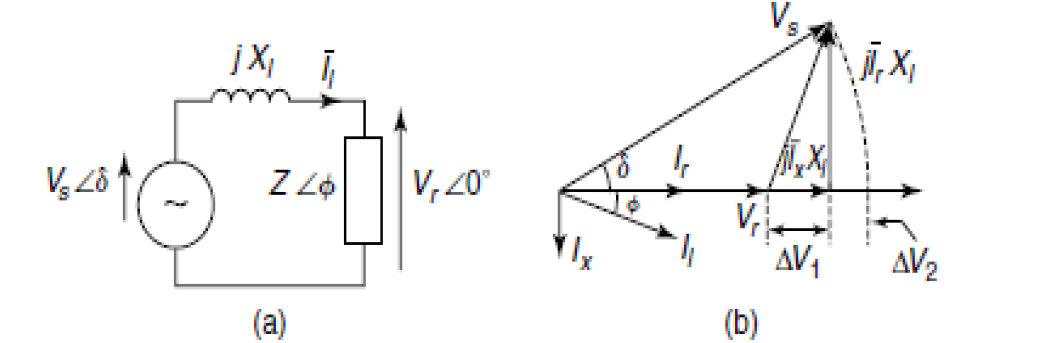
\includegraphics[width=0.6\textwidth]{Figures/figure1.png}
    \caption{Short Transmission Line Model}
\end{figure}\\
From the above figure it 
is clear that between the 
sending and the receiving end voltages,
magnitude variation as well as a
phase difference is created and the most significant part of the 
voltage drop in the line reactance is due to the reactive
component of the load current and to keep the voltages 
in the load current and to keep the voltage in the line same, we can compensate using two methods:
Load compentstion and system compensation.
\subsection*{Symmetrical line and Midpoint voltage of Symmetrical Line}
A symmetrical line is a transmission line where the sending end and receiving end voltages are equal in magnitude.
The power relations of a distributed symmatrical line, we may write, 
\begin{align}
    P_R=-P_s&=\dfrac{V^2sin\delta}{Z_csin(\beta d)}\\
    Q_r=-Q_s&=\dfrac{V^2(cos\delta-cos(\beta d))}{Z_csin(\beta d)}
\end{align}
Active and reactive powers are normalized by choosing the SIL as the base.
\subsection{Power relations and midpoint conditions in a short symmetrical uncompensated line}
Let us consider a simple two machine model where the machines are connected by a purely inductive
short transmission line as shown in the figure below:
\begin{figure}[!hb]
    \centering
    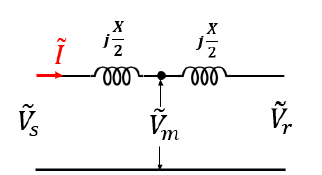
\includegraphics[width=0.6\textwidth]{Figures/figure2.png}
    \caption{Two Machine Model Connected by a Short Transmission Line}
\end{figure}\\
The phasor of the circuit can be realized as :
\begin{figure}[!hb]
    \centering
    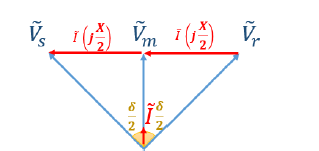
\includegraphics[width=0.6\textwidth]{Figures/figure3.png}
    \caption{Phasor Diagram of the Two Machine Model}
\end{figure}\\
Taking the midpoint voltage as reference,$V_m=V_m<0^\circ$, we can write the sending end and receiving end voltages as:
\begin{align}
    V_s&=V<\dfrac{\delta}{2}=V \left(cos\dfrac{\delta}{2}+jsin\dfrac{\delta}{2}\right)\\
    V_R&=V<-\dfrac{\delta}{2}=V \left(cos\dfrac{\delta}{2}-jsin\dfrac{\delta}{2}\right)
\end{align}
From the phasor diagram, applying parallelogram law, we can write the midpoint voltage as:
\begin{align}
    2V_m&=V_s+V_R\\
    V_m&=Vcos\dfrac{\delta}{2}<0^\circ=\dfrac{V_s+V_r}{2}
\end{align}
The current through the line is given by, 
\begin{align}
    I&=\dfrac{V_s-V_r}{jX}\\
    &=\dfrac{2V}{X}sin\dfrac{\delta}{2}<0^\circ
\end{align}
For lossless line, the active power at the sending and receiving end are given by,
\begin{align}
    P&=V_mI=\dfrac{V^2}{X}sin\delta
\end{align}
The reactive power is :
\begin{equation}
Q_s=-Q_r=VIsin(\delta/2)=\dfrac{V^2}{X}(1-\cos(\delta))
\end{equation}
The voltage profile of a symmetrical line for varying load is as shown in figure: 
\begin{figure}[!hb]
    \centering
    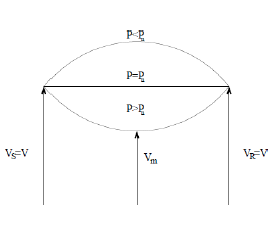
\includegraphics[width=0.5\textwidth]{Figures/figure4.png}
    \caption{Voltage Profile of a Symmetrical Uncompensated Transmission Line}
\end{figure}\\
The power curve after compensation is as shown : 
\begin{figure}[!hb]
    \centering
    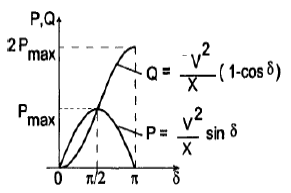
\includegraphics[width=0.6\textwidth]{Figures/figure5.png}
    \caption{Power Curve after Midpoint Compensation}
\end{figure}\\
It is seen that the reactive power compensated is twice the active power transferred.
\section{Observation}
\subsection*{Uncompensated Transmission Line}\
The Simulink model of an uncompensated transmission line is as shown below:
\begin{figure}[!hb]
    \centering
    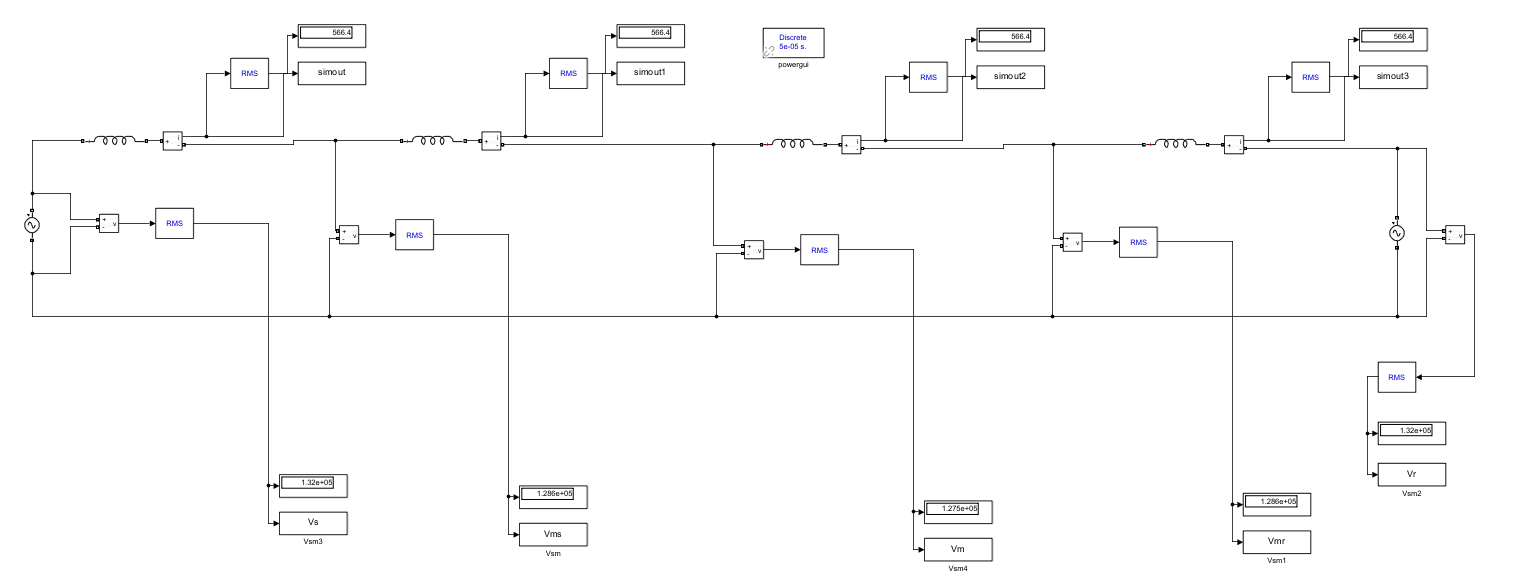
\includegraphics[width=1\textwidth,height=0.56\textwidth]{Figures/figure7.png}
    \caption{Simulink Model of Uncompensated Transmission Line}
\end{figure}
\newpage
The voltage profile of the uncompensated transmission line is as shown below:
\begin{figure}[h]
    \centering
    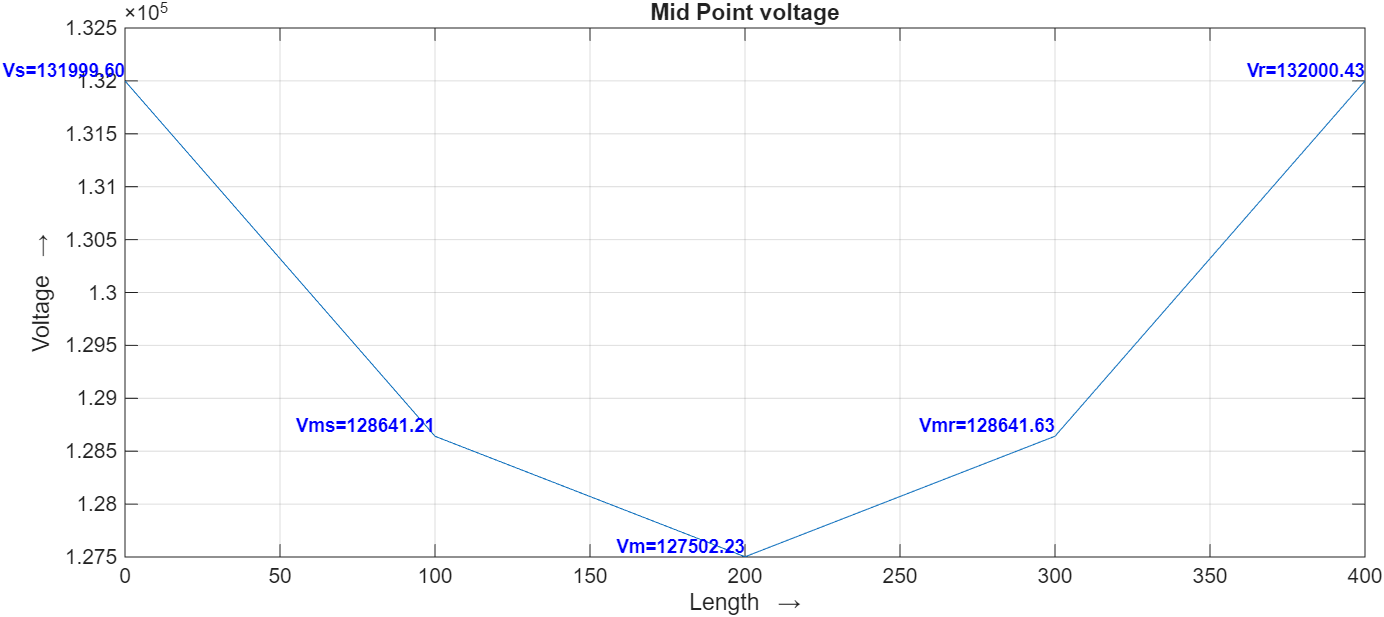
\includegraphics[width=1\textwidth]{Figures/figure9.png}
    \caption{Voltage Profile of Uncompensated Transmission Line}
\end{figure}
\subsection*{Compensated Transmission Line}
The Simulink model of a compensated transmission line is as shown below:
\begin{figure}[!hb]
    \centering
    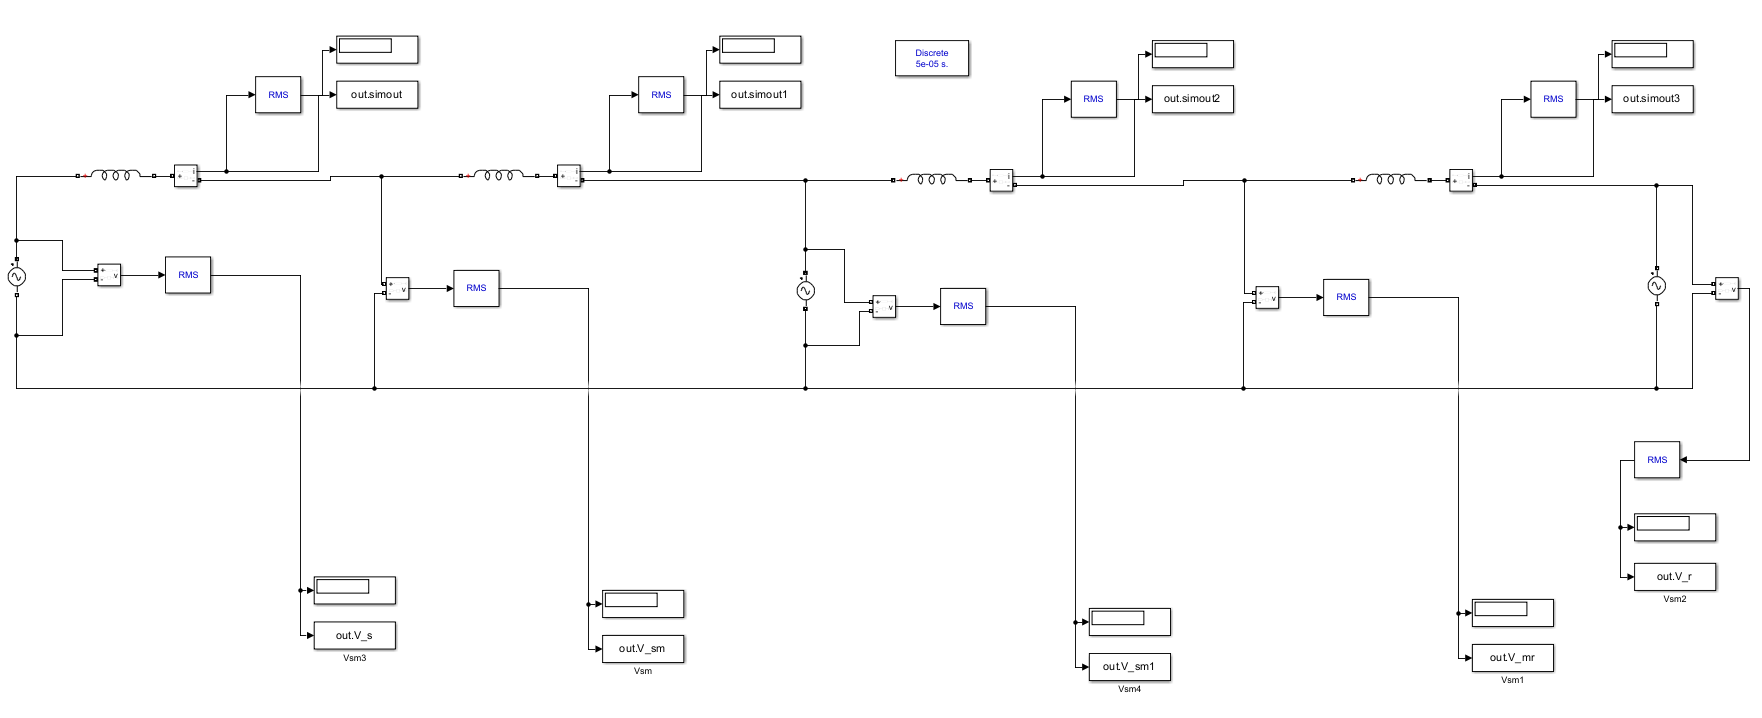
\includegraphics[width=1\textwidth,height=0.6\textwidth]{Figures/figure6.png}
    \caption{Simulink Model of Compensated Transmission Line}
\end{figure}
\newpage
The voltage profile of the compensated transmission line is as shown below:
\begin{figure}[!hb]
    \centering
    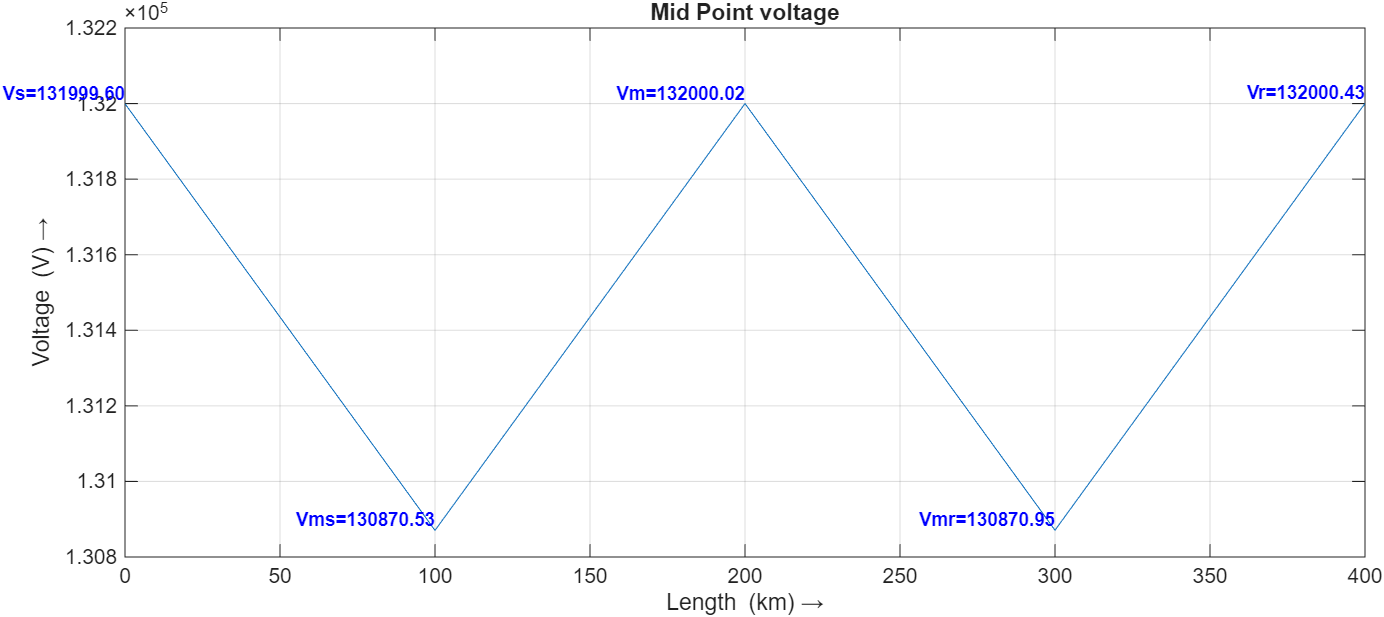
\includegraphics[width=1\textwidth]{Figures/figure8.png}
    \caption{Voltage Profile of Compensated Transmission Line}
\end{figure}
\subsection*{Compensation of voltage at Quarter Points of the transmission Line}
The Simulink model of compensation at quarter points of the transmission line is as shown below:
\begin{figure}[!hb]
    \centering
    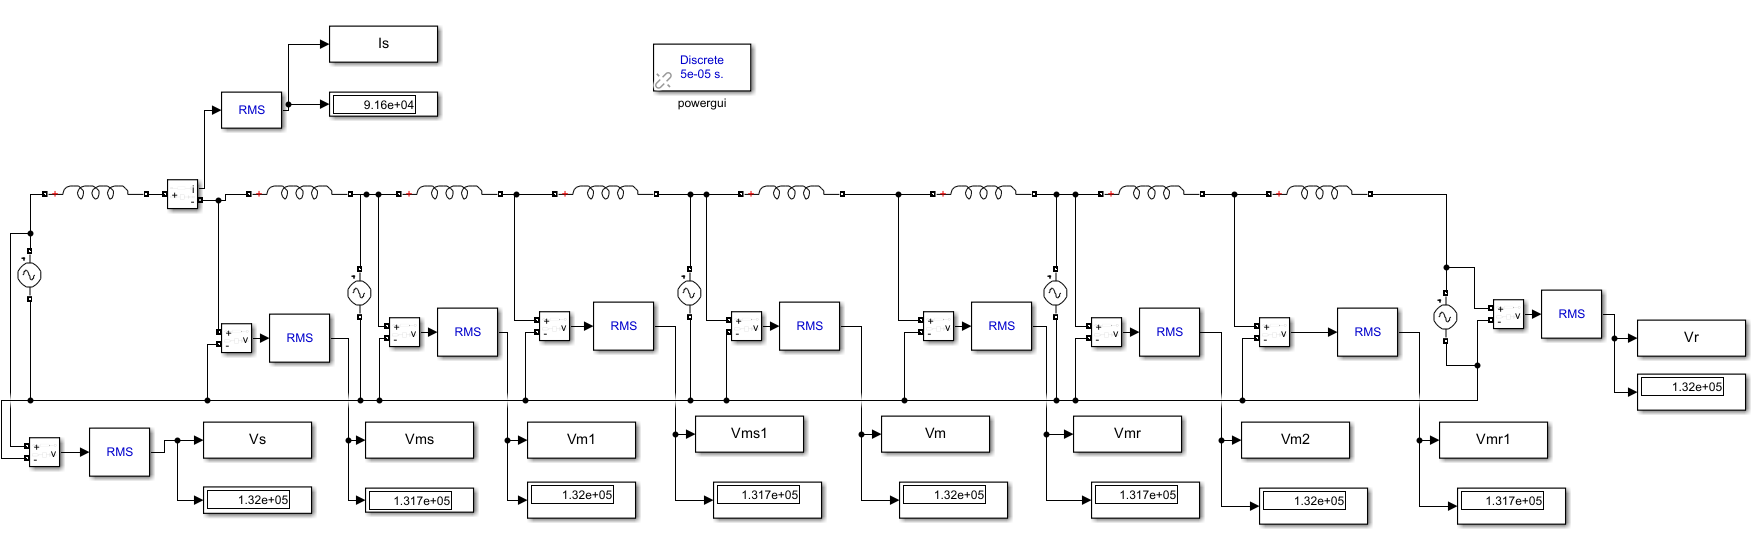
\includegraphics[width=1.05\textwidth,height=0.56\textwidth]{Figures/figure10.png}
    \caption{Simulink Model of Compensation at Quarter Points of the Transmission Line}
\end{figure}
\newpage
The voltage profile of the compensated transmission line at quarter points(\textbf{jX/4}) is as shown below:
\begin{figure}[!hb]
    \centering
    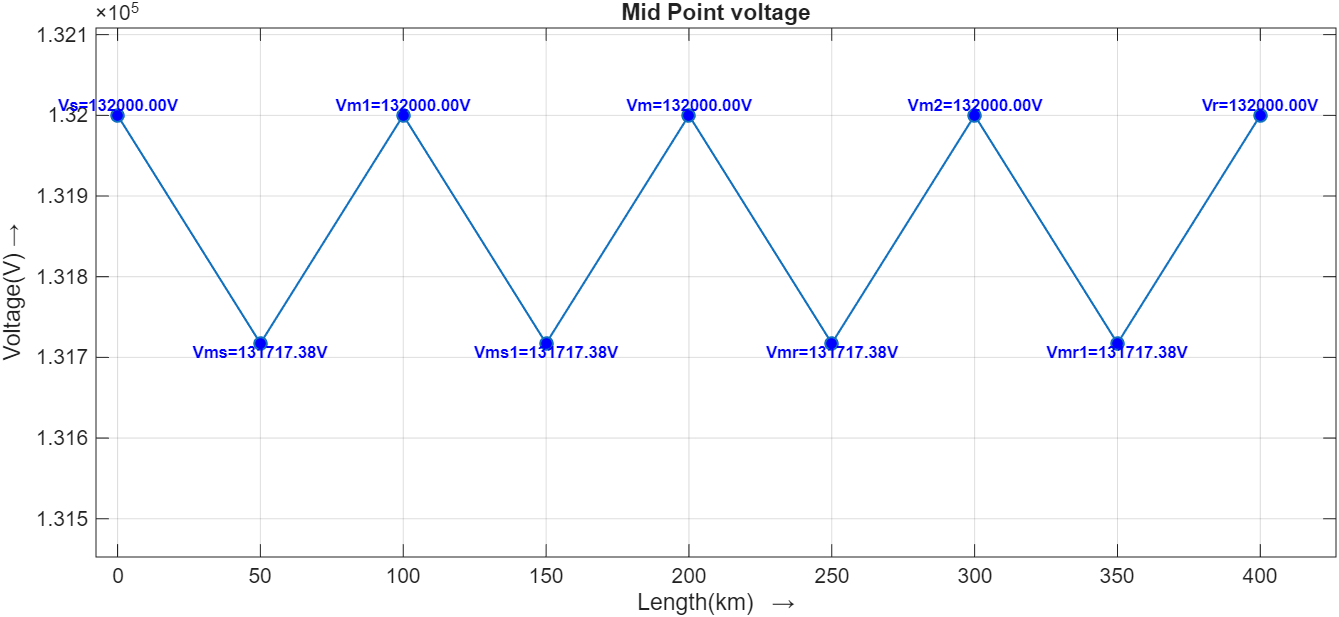
\includegraphics[width=1\textwidth]{Figures/figure11.png}
    \caption{Voltage Profile of Compensated Transmission Line at Quarter Points(jX/4)}
\end{figure}
\section{Discussion}
For the symmetrical uncompensated line, the voltage decreases 
smoothly from both ends towards the centre, forming a 
U shaped voltage profile. The midpoint voltage is lower than both the sending and receiving end voltages due to the voltage drop across the line reactance.\\[0.2cm]
With midpoint compensation of jX/2, half of the line reactance is cancelled at the centre, so the midpoint voltage rises close to the rated value while two smaller voltage dips appear symmetrically on either side. The voltage profile becomes M-shaped, indicating improved regulation and higher power-transfer capability compared to the uncompensated case.\\[0.2cm]
When the compensation is split into two jX/4sections, reactive support is distributed along the line, producing an almost flat voltage profile with only small ripples. This arrangement gives the best voltage regulation and stability margin, showing that distributed series compensation is more effective than concentrating it at a single point.
\section{Conclusion}
Hence, we saw that compensating voltages at different points significantly improved the voltage profile of the transmission line.
\end{document}